\chapter{Test}
\label{chap:test}

\section{Test ``Analisi assistita''}

\subsection{Sito web: SudokuWorld}

\subsubsection{Total Validator}
\begin{figure}[H]
    \centering
    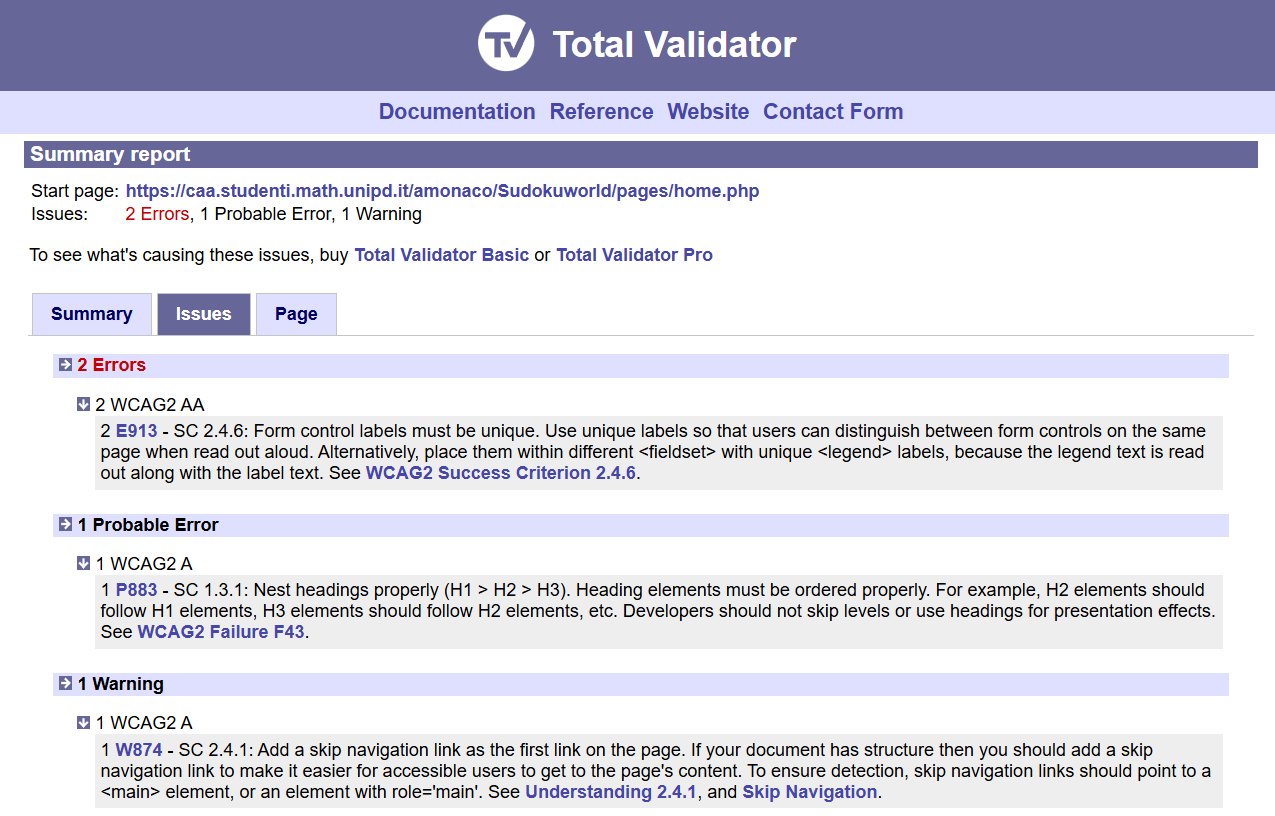
\includegraphics[width=0.7\linewidth, alt={Screenshot dell'analisi di Total Validator sul sito web SudokuWorld}]{img/TV_sudoku.png}
    \caption{Analisi di Total Validator sul sito web SudokuWorld}\label{fig:TV_sudoku}
\end{figure}

\noindent Come visibile nella figura \ref{fig:TV_sudoku} è possibile vedere che lo strumento TV trova ben 15 errori di accessibilità.\\
Gli errori principali sono: 
\begin{itemize}
    \item E913 - SC 2.4.6: Le etichette dei controlli dei form devono essere univoche. Utilizzare etichette univoche consente agli utenti di distinguere i vari controlli presenti sulla stessa pagina quando vengono letti da uno screen reader. In alternativa, è possibile inserirli all’interno di diversi <fieldset> con <legend> univoci, poiché il testo del <legend> viene letto insieme all’etichetta del controllo. Vedi WCAG2 Success Criterion 2.4.6.
    \item E31 - Sono stati rilevati errori ortografici. Le parole non presenti nel dizionario vengono evidenziate e accompagnate da un elenco di possibili sostituzioni (in parentesi).
    \item P883 - SC 1.3.1: Nidificare correttamente le intestazioni (H1 > H2 > H3). Gli elementi di intestazione devono essere ordinati in modo gerarchico. Ad esempio, un elemento H2 dovrebbe seguire un H1, un H3 dovrebbe seguire un H2, e così via. Gli sviluppatori non devono saltare livelli né utilizzare le intestazioni solo per scopi di presentazione. Vedi WCAG2 Failure F43.
\end{itemize}

\subsubsection{Lighthouse}
Lo strumento lighthouse mostra che accessibilità è al 100\% ... (figura ...)
\begin{figure}[H]
    \centering
    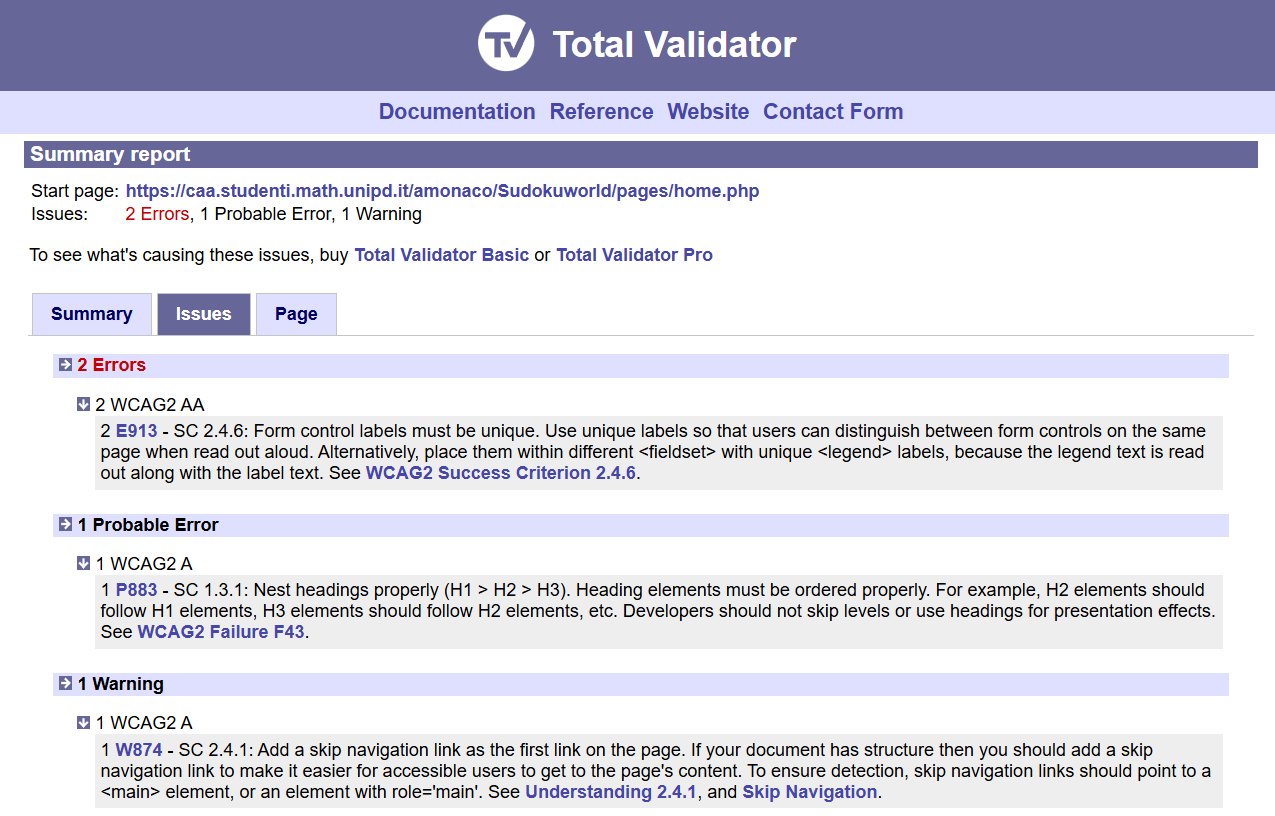
\includegraphics[width=0.7\linewidth, alt={Screenshot dell'analisi di Total Validator sul sito web SudokuWorld}]{img/TV_sudoku.png}
    \caption{Analisi di Total Validator sul sito web SudokuWorld}\label{fig:TV_sudoku}
\end{figure}

\subsubsection{SviluppAbile}
\noindent Di seguito vengono riportati i test effettuati con l'estensione \textit{SviluppAbile}.

\subsubsection*{\texttt{Il mio codice HTML rispetta le linee guida WCAG?}}
\begin{adjustwidth}{1cm}{1cm}
\noindent {\footnotesize Il tuo codice HTML sembra essere in parte conforme alle linee guida WCAG (Web Content Accessibility Guidelines), ma potrebbe migliorare ulteriormente per garantire una maggiore accessibilità. Alcune aree che richiedono ulteriore attenzione includono:\\
- L'attributo `aria-label` non è utilizzato in modo coerente nei controlli di navigazione.\\
- Le etichette dei pulsanti "Cerca" e "Profilo" potrebbero essere più descrittive.\\
Tuttavia, il tuo codice include molti elementi positivi come l'utilizzo di `alt` per immagini, la presenza di un titolo (`<title>`) e di metatag di descrizione (`<meta name="description">`). Questi sono passaggi fondamentali per migliorare la comprensione del contenuto da parte dei motori di ricerca e degli assistenti.\\
Per garantire una maggiore accessibilità, considera di applicare ulteriormente le linee guida WCAG 2.1, che offrono standard e raccomandazioni per creare esperienze web più inclusive.\\
La pagina non rispetta la norma W3C WCAG 2.1 che richiede di nidificare correttamente le intestazioni. Non sono presenti elementi HTML con attributo "h1", mentre ci sono intestazioni con grado inferiore.}
\end{adjustwidth}

\subsubsection*{\texttt{xx}}
\noindent {\footnotesize aaa}

\subsubsection*{\texttt{xx}}
\noindent {\footnotesize aaa}

\subsubsection{Resoconto finale}
\noindent SviluppAbile riesce a riconoscere i principali problemi di struttura semantica e form.\\
Ha individuato gli stessi problemi evidenziati da TV, in particolare:
\begin{enumerate}
    \item Struttura delle intestazioni (WCAG 1.3.1): in diverse pagine è stata rilevata la mancata nidificazione corretta degli heading (<h1> > <h2> > <h3>).
    \item Accessibilità dei form: problemi relativi a etichette non uniche e campi privi di label/aria-label sono stati segnalati da entrambe le analisi.
    \item Mancanza di pulsanti submit o pulsanti non correttamente etichettati.
\end{enumerate}

\vspace{0.5cm}
\noindent \textbf{PRO:}\\
\noindent Rispetto alla valutazione di TV, \textit{SviluppAbile} fornisce descrizioni dettagliate dei problemi e suggerimenti di correzione con esempi di codice, non limitandosi alla sola segnalazione dell’errore. Inoltre individua aspetti migliorabili non segnalati da TV, come L’uso non coerente di aria-label nei controlli di navigazione, etichette di pulsanti poco descrittive, mancanza di alternative testuali esaustive per immagini già dotate di alt.\\
Rispetto allo strumento Lighthouse, il quale assegna un punteggio del 100\% sull'accessibilità, \textit{SviluppAbile} individua errori e aiuta a correggerli.\\
Continuando a fare domande nella chat si possono approfondire man-mano i vari aspetti dell’accessibilità, cosicché lo sviluppatore possa migliorare la propria pagina web.

\vspace{0.5cm}
\noindent \textbf{CONTRO:}\\
\noindent Rispetto alla valutazione di TV e di un esperto di accessibilità web, \textit{SviluppAbile} non segnala alcuni dettagli di esperienza utente (ad esempio mancanza di presentazione del sito, estetica troppo predefinita, assenza di padding/margini); problemi di navigazione post-login/logout o di comportamento del carosello, che sono più legati alla logica di funzionamento che al solo HTML.\\
\textit{SviluppAbile} necessita di domande specifiche e in alcuni casi del caricamento degli errori individuati da altri strumenti (Total Validator) per l’individuazioni di alcuni errori.\\
Inoltre, essa non ha accesso al file di stile, quindi non può controllare la parte relativa ai colori/link visitati.

\vspace{0.5cm}
\noindent \textbf{CONCLUSIONE:}\\
\noindent Il confronto evidenzia che \textit{SviluppAbile} è efficace nell’individuare gran parte delle non conformità WCAG 2.1 di tipo tecnico e fornisce un supporto pratico agli sviluppatori grazie ai suggerimenti di modifica.\\
La valutazione del sito web effettuata durante il concorso, seppur meno dettagliata sul piano tecnico, integra invece aspetti legati alla fruibilità reale del sito e alla presentazione dei contenuti, che attualmente richiedono ancora un’analisi manuale.


\section{Test ``Modalità guidata''}